% fig_wires.tex -- wire vs reg, and module hierarchy
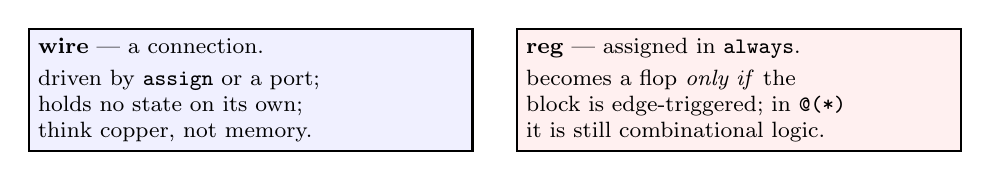
\begin{tikzpicture}[font=\footnotesize]
  \node[draw, thick, fill=blue!6, text width=5.4cm, align=left] at (0,0)
    {\textbf{wire} --- a connection.\\[2pt]
     driven by \texttt{assign} or a port;\\
     holds no state on its own;\\
     think copper, not memory.};
  \node[draw, thick, fill=red!6, text width=5.4cm, align=left] at (6.2,0)
    {\textbf{reg} --- assigned in \texttt{always}.\\[2pt]
     becomes a flop \emph{only if} the\\
     block is edge-triggered; in \texttt{@(*)}\\
     it is still combinational logic.};
\end{tikzpicture}
